%% Dewey and a re-evaluation of retrieval-augmented scholarly QA on DBLP-QA.
%% IEEE conference template (IEEEtran); also compiles as-is on Overleaf (upload main.tex + references.bib).
%% Built by .github/workflows/paper.yml (latexmk, pdflatex + bibtex); every number below comes from
%% the run artefacts of `python -m chat.cli dblpqa ...` and `chat.cli evaluate|qa|scenarios`
%% (chat/chat/dblpqa*.py, evaluate.py, qa.py, scenarios.py).
\documentclass[conference]{IEEEtran}
\IEEEoverridecommandlockouts

\usepackage{cite}
\usepackage{amsmath,amssymb}
\usepackage{graphicx}
\usepackage{textcomp}
\usepackage{xcolor}
\usepackage{booktabs}
\usepackage{url}
\usepackage{pgfplots}
\pgfplotsset{compat=1.18}
\usetikzlibrary{positioning,arrows.meta}

%% categorical slots 1-4 of the validated reference palette (light surface), one per answering system;
%% markers differ too, so the figure survives grey-scale printing and colour-vision deficiencies
\definecolor{seriesA}{HTML}{2A78D6}   % gpt-4.1
\definecolor{seriesB}{HTML}{EB6834}   % gpt-4.1-mini
\definecolor{seriesC}{HTML}{1BAF7A}   % Mistral-7B
\definecolor{inkmuted}{HTML}{52514E}
\definecolor{gridline}{HTML}{E4E3DF}

%% marks text that waits for a run still in progress
\newcommand{\pending}[1]{\textcolor{red}{[pending: #1]}}
\newcommand{\ci}[2]{{\scriptsize[#1,\,#2]}}
\newcommand{\dq}{DBLP-QA}
\newcommand{\fresh}{DBLP-QA-Fresh}

\begin{document}

\title{Beyond Retrieve-then-Read: Dewey, a Tool-Calling Assistant for dblp, and a Re-evaluation of
DBLP-QA}

\author{\IEEEauthorblockN{Hadi Ghazi}
\IEEEauthorblockA{\textit{Lebanese University}\\
hadigghazi@gmail.com}}

\maketitle

\begin{abstract}
RAGScholar answers questions about computer-science papers by retrieving abstracts with BM25 and
reading them with a small language model; its benchmark, DBLP-QA, was graded by hand. We build Dewey, an
assistant that answers questions about dblp by calling tools over the whole dump, and evaluate both
automatically: a language-model judge applies the benchmark's 0--2 scale only after passing control
checks, and a second judge from another model family re-grades the main results. First, we re-run every
experiment of the original study. Given the right abstract, every model scores at least 1.96 of 2 under
the primary judge, so what decides the score is finding the paper: today's public search services put it
among the top five for 58\% of \dq{} questions and for 89\% of 100 new questions about 2025--2026 papers,
and the gain from retrieval follows that rate. Several of the original findings hold under automatic
grading; \pending{which do not}. Second, we give Dewey this retrieval as one of its tools. On
RAGScholar's own questions, Dewey scores \pending{X} against \pending{Y} for RAGScholar's best
configuration re-implemented on the same candidates and graded by the same judge, and matches a fixed
pipeline that uses its own model \pending{confirm}. On 70 questions about dblp's records, such as who
wrote a paper, how many papers a venue published in a year or how many people share a name, checked
against values computed from the dump without any judge, Dewey answers \pending{N} and a RAGScholar-style
pipeline \pending{M}. Retrieving the wrong papers seems to cost points only when answers are graded
against a single reference answer.
\end{abstract}

\begin{IEEEkeywords}
retrieval-augmented generation, tool-calling agents, scholarly question answering, dblp,
LLM-as-a-judge, benchmark evaluation
\end{IEEEkeywords}

%% ===================================================================================================
\section{Introduction}

Retrieval-augmented generation (RAG) conditions a language model's answer on documents retrieved for
the question~\cite{lewis2020rag,gao2023ragsurvey}. For scholarly information access it promises answers
that can be traced to publications rather than to a model's memory. Neekhra, Nilles and Schenkel recently
introduced DBLP-QA, a benchmark of 50 question--answer pairs written from abstracts of papers indexed by
dblp~\cite{ley2009dblp}, together with RAGScholar, a system that retrieves abstracts with Lucene BM25 and
answers with instruction-tuned models from 0.78B to 14.7B parameters~\cite{neekhra2026ragscholar}. They
compared ten ways of building the context, from single abstracts to concatenated abstracts and
concatenated answers, and rated the answers by hand on a 0--2 scale; the best configuration, Mistral-7B
with the top five abstracts concatenated, scored 1.74, against 0.80 without retrieval.

RAGScholar answers one kind of question: what a paper says. Much of what people ask a bibliography is of
other kinds: who wrote a paper and where it appeared, how many papers a person or a venue has, who
publishes most where, who works with whom, how many different people share a name. A system that
retrieves five abstracts and reads them has nothing to count, rank or tell people apart with. We built
Dewey, the assistant of a dblp exploration website, for these questions: a tool-calling
agent~\cite{schick2023toolformer,yao2023react} whose tools query the full dblp dump. This paper asks
whether Dewey can also do what RAGScholar does, and how to show that without grading by hand.

Answering that requires evaluating RAGScholar's setting again. The models it evaluated are small, so it
is unclear how much of the benchmark a current model answers without retrieval, and whether from general
knowledge or from having read the papers. Retrieval was evaluated in a closed world: the questions were
sampled from the very collection that was indexed, and that collection is no longer fully available, so
the setting cannot be rebuilt. Each question has one reference answer taken from one abstract, which may
penalise correct answers drawn from other papers. And ratings made by hand cannot be re-run when a system
changes. Our research questions are:

\begin{itemize}
\item \textbf{RQ1:} What do current models score without retrieval and given the source abstract, and
  where does their prior knowledge come from?
\item \textbf{RQ2:} How often can the source paper, or any abstract that answers the question, be
  retrieved in an open-world setting today?
\item \textbf{RQ3:} Do the original study's findings about context construction and model choice hold
  under automatic grading?
\item \textbf{RQ4:} How does Dewey, given RAGScholar's retrieval as a tool, compare with RAGScholar on
  RAGScholar's own questions?
\item \textbf{RQ5:} How do the two compare on questions about dblp's records?
\item \textbf{RQ6:} How robust are these conclusions to the grading protocol and the judge?
\end{itemize}

Our contributions are: (i)~Dewey, a tool-calling assistant over the dblp dump with a content tool built
from this study's findings, and its own evaluation (Section~\ref{sec:dewey}); (ii)~an automatic
re-run of every experiment of the original study, with a judge gated by controls, a second judge from
another family and paired statistics, which tests its findings one by one; (iii)~\fresh{}, 100 questions
built the same way, automatically, about papers published after the models' training cutoffs;
(iv)~an open-world reconstruction of retrieval from public services, with frozen candidate pools, and
evidence that retrieval success, not generation, now decides performance; (v)~a head-to-head comparison
of Dewey with a re-implementation of RAGScholar's pipeline, on its questions and on 70 questions about
dblp's records scored without a judge; and (vi)~evidence that what retrieving the wrong papers appears to
cost depends on both the grading protocol and the judge. Everything runs on one CPU virtual machine; all
API calls together cost \pending{total} US dollars.

%% ===================================================================================================
\section{Related Work}

\textbf{Scholarly QA over dblp.} DBLP-QuAD~\cite{banerjee2023dblpquad} asks questions over the dblp
knowledge graph (authors, venues, years), answered by translating them into queries; our record questions
(Section~\ref{sec:structured}) follow its question types. DBLP-QA~\cite{neekhra2026ragscholar} instead
asks about the content of papers, answerable from their abstracts. Dewey covers both kinds.

\textbf{Tool-calling assistants.} Language models can learn to call external
tools~\cite{schick2023toolformer} and to interleave reasoning with actions~\cite{yao2023react}. Dewey is
such an agent; its tools are typed queries over a bibliographic database, and retrieval over abstracts is
one tool among them rather than the whole system.

\textbf{Retrieval, distractors and selective retrieval.} Irrelevant context can mislead language
models~\cite{shi2023distracted}, the position of the relevant passage matters~\cite{liu2024lost}, and
the effect of non-relevant documents in RAG is not uniformly negative~\cite{cuconasu2024noise}. Whether
to retrieve at all depends on how well a model already knows the answer~\cite{mallen2023trust}, which
motivates adaptive and self-reflective schemes such as Self-RAG~\cite{asai2024selfrag},
CRAG~\cite{yan2024crag} and Adaptive-RAG~\cite{jeong2024adaptiverag}. Our gated condition is a simple
member of this family.

\textbf{Evaluation.} LLM judges agree well with humans on many tasks but have biases, including a
preference for their own generations~\cite{zheng2023judge,panickssery2024selfpref}. Lexical and
single-reference evaluation underestimates open-domain QA systems whose correct answers are phrased
differently or differ in content~\cite{kamalloo2023evaluating}; we find the same effect in a RAG
setting. Benchmarks built from public text may be contaminated by pre-training
data~\cite{sainz2023contamination}; a set built from papers newer than the models avoids this.

%% ===================================================================================================
\section{Dewey}
\label{sec:dewey}

\begin{figure}[t]
\centering
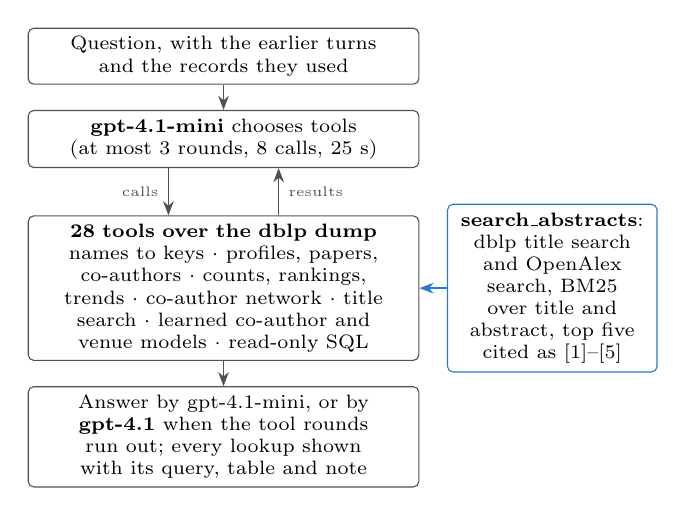
\begin{tikzpicture}[
  font=\scriptsize, node distance=3.2mm,
  box/.style={draw=inkmuted, rounded corners=2pt, align=center, text width=4.75cm, inner sep=3pt},
  new/.style={draw=seriesA, rounded corners=2pt, align=center, text width=2.45cm, inner sep=3pt},
  arr/.style={-{Stealth[length=1.8mm]}, draw=inkmuted, line width=0.5pt}]
\node[box] (q) {Question, with the earlier turns and the records they used};
\node[box, below=of q] (r) {\textbf{gpt-4.1-mini} chooses tools\\(at most 3 rounds, 8 calls, 25 s)};
\node[box, below=6mm of r] (t) {\textbf{28 tools over the dblp dump}\\names to keys $\cdot$ profiles, papers,
  co-authors $\cdot$ counts, rankings, trends $\cdot$ co-author network $\cdot$ title search
  $\cdot$ learned co-author and venue models $\cdot$ read-only SQL};
\node[box, below=of t] (a) {Answer by gpt-4.1-mini, or by \textbf{gpt-4.1} when the tool rounds run
  out; every lookup shown with its query, table and note};
\node[new, right=3.5mm of t] (s) {\textbf{search\_abstracts}: dblp title search and OpenAlex
  search, BM25 over title and abstract, top five cited as [1]--[5]};
\draw[arr] (q) -- (r);
\draw[arr] ([xshift=-7mm]r.south) -- node[left, font=\tiny, text=inkmuted] {calls} ([xshift=-7mm]t.north);
\draw[arr] ([xshift=7mm]t.north) -- node[right, font=\tiny, text=inkmuted] {results} ([xshift=7mm]r.south);
\draw[arr] (t) -- (a);
\draw[arr, draw=seriesA] (s.west) -- (t.east);
\end{tikzpicture}
\caption{Dewey: a tool-calling agent over the dblp dump. Blue: the content tool built from this
study's findings (Section~\ref{sec:content}).}
\label{fig:dewey}
\end{figure}

Dewey is the assistant of dblp Explorer, a public website for exploring the dblp dump (Fig.~\ref{fig:dewey}).
It is a tool-calling agent rather than a document-retrieval pipeline. gpt-4.1-mini reads the question
and the earlier turns, and calls tools, at most three rounds and eight calls within 25 seconds; once it
stops calling tools it writes the answer itself, and gpt-4.1 writes it instead when the tool rounds or
the time budget run out after the second round. Of its 28 tools, 22 query the dump through DuckDB: they
resolve author and venue names to dblp keys, tolerating misspellings and names written in other scripts;
return profiles, paper lists, co-authors, counts, rankings and time series; place authors in the
co-authorship network by four centrality measures; and run read-only SQL. The others call the project's
services: a title search, two learned models that suggest likely co-authors and venues, the models'
measured accuracy, the project's documentation, and the content tool below. Table~\ref{tab:capabilities}
sets the kinds of question this covers beside what RAGScholar's design can answer.

Every tool returns its counting rules with its rows (whether preprints are included, whether
disambiguation bins are excluded), totals come from their own aggregate rather than from the length of a
capped list, and a failed lookup is an explicit refusal rather than an empty table, which a language
model reads as zero. The answer shows every lookup with its arguments, table, note and a link to the
matching dashboard page, so each number can be traced to a query. The system prompt forbids stating a
number, name or ranking that no tool returned, and tells Dewey to decline questions the data cannot
answer, such as citation counts, affiliations of papers or awards; this is an instruction, measured
below, not a check run before an answer is shown. Follow-up questions work because each answer is
remembered with the records its tools returned, so ``the second one'' resolves to a key rather than a
guess.

\begin{table}[t]
\caption{What each system can answer. RAGScholar: as its paper describes it (BM25 over title and abstract,
the top abstracts given to the model, one question at a time). Dewey: the gold-set cases of each kind
(Section~\ref{sec:deweyeval}) and the measurements of Sections~\ref{sec:rq4}--\ref{sec:rq5}.}
\label{tab:capabilities}
\centering\scriptsize
\setlength{\tabcolsep}{2.4pt}
\begin{tabular}{p{2.55cm}p{1.75cm}p{3.35cm}}
\toprule
Question & RAGScholar & Dewey \\
\midrule
What a paper says & yes & content tool, cited [1]--[5] (RQ4) \\
A paper's venue, year, authors & if retrieved & record lookup (RQ5; gold set) \\
Counts with filters & no & counted in the dump (RQ5; gold set) \\
Rankings, superlatives & no & precomputed or live (RQ5; gold set) \\
Trends over years & no & yearly series (gold set) \\
Co-authors, joint papers & no & co-author tools (RQ5; gold set) \\
Position in the co-author network & no & four centrality measures (gold set) \\
People who share a name & no & numbered pages and bins (RQ5; scenarios) \\
Follow-ups (``the second one'') & no & records carried between turns (gold set) \\
Likely co-authors or venues & no & two learned models (gold set) \\
Questions the data cannot answer & not stated & declined (gold set) \\
\bottomrule
\end{tabular}
\end{table}

\textbf{Title search.} The search tool fuses BM25 over titles with cosine similarity of
text-embedding-3-large vectors by reciprocal rank fusion~\cite{cormack2009rrf}, weighting BM25 by how
much of the query the best title match covers, down to zero for descriptions in other words. It indexes
dblp's 5.36 million journal and conference papers from 2010 on; older papers and other record kinds are
reached only by an exact-word fallback.

\subsection{The content tool}
\label{sec:content}

Until this study Dewey declined questions about what papers say, since dblp holds titles, not abstracts.
Its content tool, \emph{search\_abstracts}, is the retrieval this study found best
(Section~\ref{sec:rq2}), built from the same code: three searches run in parallel (Dewey's title search,
top 50; OpenAlex~\cite{priem2022openalex} keyword search with the question's words OR-ed, top 50; and
OpenAlex semantic search over titles and abstracts, top 50); OpenAlex works are kept only where dblp has
the paper, mapped by DOI, arXiv identifier or exact normalised title through an index built once per
dump (7.37 million DOIs and 410{,}000 arXiv identifiers, built in 42 seconds); papers without an abstract
get one by DOI, or from their preprint or published twin; and BM25 over title and abstract ranks the
pool. The five best are returned, numbered, and the prompt asks Dewey to answer from them, end every
sentence that uses one with its number, say when none addresses the question, and only then add general
background, marked as such. Results are cached per query, OpenAlex calls are capped per day within its
free allowance, and a source that is slow is cut off at 12 seconds and reported as degraded. A switch
restores the old behaviour, which the evaluation uses as a baseline.

\subsection{Dewey's own evaluation}
\label{sec:deweyeval}

Three test suites check Dewey before the comparisons below.

\textbf{Gold set.} \pending{72} questions, each naming the tools that must be called (and, where it
matters, their arguments and that they succeeded), cover lookups, superlatives, counts, trends,
multi-hop questions, namesakes, predictions, the co-authorship network, follow-ups, a question in Arabic,
questions about paper content and \pending{10} questions outside the data that must be declined. On its
latest run Dewey called the right tools for \pending{x of y} in-scope questions and declined all
\pending{10} out-of-scope ones; an offline lint, which looks for every number of an answer among the tool
results, the call arguments and the question, allowing rounding and skipping years and counts up to 24,
found no number without a source. The median answer took \pending{2.6} seconds and the run cost
\pending{US\$0.3}. These are process checks written by the developer, not answer accuracy.

\textbf{Dashboard checks.} \pending{24} checks run the tools without a model and compare their numbers with
the dashboard's own endpoints (author and venue profiles, namesake counts, yearly series), test
invariants (a total does not change with the row cap; filters only narrow; kinds sum to the total; bins
are never people) and behaviour (every tool answers within four seconds, bad input is refused, ten SQL
injection attempts are refused); \pending{24/24} pass.

\textbf{Instructor scenarios.} \pending{27} questions about one person who shares a name with another
dblp author, asked the ways a user would ask them (by affiliation, misspelled, surname only, in Arabic,
as follow-ups); a scenario also fails if any lookup used the namesake. \pending{26/27} pass.

\textbf{Search.} Asked for a paper with one distinctive title word replaced by a synonym (666 queries),
the hybrid search returns it first for 99\%. Asked with a description that avoids the title's
distinctive words (56 queries written by gpt-4.1-mini), word matching finds none of the papers in its top
ten and embeddings find 16\%, the weakness of BM25 that the original study names; before re-embedding
5.36 million titles, a pilot on 177 such queries chose text-embedding-3-large over the previous model
(better on 135, worse on 22).

%% ===================================================================================================
\section{Evaluation Method}

\subsection{Benchmarks}

\textbf{\dq{}} has 50 questions, each with a 1--3 sentence reference answer, the dblp key of its source
paper and its Semantic Scholar corpus id. We fetch source abstracts from Semantic
Scholar~\cite{kinney2023s2}, falling back to arXiv, OpenAlex and Crossref; 46 of the 50 are available.

\textbf{\fresh{}} separates knowledge of a field from memory of particular papers. We sample, with a
fixed seed, journal and conference papers in dblp published in 2025 or later, after GPT-4.1's June 2024
training cutoff and Mistral-7B v0.1's 2023 release, excluding preprints, and fetch their abstracts by
DOI. gpt-4.1 writes one question per abstract with a 1--3 sentence answer taken from it, using four \dq{}
pairs as style examples. A question is kept only if gpt-4.1-mini's answer from the abstract scores 2; of
the 102 questions that reached this check, 100 were kept, so counting the two removed questions as wrong
would lower no model's oracle mean below 1.92. No question is filtered on closed-book answers, which would
make the models fail by construction. The build cost US\$0.36.

\textbf{Record questions.}
\label{sec:structured}
Seventy questions about dblp's records, ten of each of seven kinds that follow DBLP-QuAD's question
types~\cite{banerjee2023dblpquad}: a paper's venue and year; its authors; the number of publications of a
person; the number of papers of a venue in a year; a venue's most prolific author; the number of papers
two people wrote together; and the number of different people who share a name. They are drawn from the
current dump with a fixed seed, and every reference answer is computed by SQL over the raw dblp file, not
through Dewey's tools or the database they read, then frozen before any system answers. Only people with
a single author page that carries a single name and is not a disambiguation bin are named, and a venue's
top author is asked only when there is a clear winner. Scoring needs no judge: the reference number must
appear in the answer; for a paper, its year and venue, where the venue counts if every word of dblp's
abbreviation begins a word of the answer in order (so ``International Journal of Medical Informatics''
names ``Int. J. Medical Informatics''); for authors, every surname; for a top author, every name.

\subsection{Systems and conditions}

On \dq{} and \fresh{}:
\begin{itemize}
\item \textbf{Closed-book:} the question alone.
\item \textbf{Oracle:} the question with its source abstract.
\item \textbf{RAG:} the question with retrieved abstracts, in the original study's ten context variants:
  no context, each of the top five abstracts on its own (A1--A5), the top three or five concatenated
  (Top-3/5-CD), and an answer written from each of the top three or five, combined into one answer
  (Top-3/5-CA). Top-5-CD, the original study's best, is the main condition.
\item \textbf{Selective RAG:} Top-5-CD with a \emph{permissive} prompt (the abstracts may not be
  relevant; if none addresses the question, answer from what you know), or \emph{gated} (a separate
  gpt-4.1-mini call keeps only the abstracts that address the question; with none kept, closed-book).
\item \textbf{Dewey}, given each question as a user would type it: \emph{as deployed}, with live
  searches; \emph{on the frozen pool}, where the content tool ranks the study's frozen candidates for the
  question instead of searching, so Dewey sees what the fixed pipeline saw; and \emph{before the content
  tool}, with the tool switched off and the old rule back.
\end{itemize}
The \emph{RAGScholar configuration} is Mistral-7B with Top-5-CD on our candidates. It re-implements the
original study's best system, not the system itself: the original prompt is unpublished (ours asks for one
to three sentences), our model is 4-bit quantised on a CPU, and the candidates come from our open-world
pool. On the record questions, the \emph{RAGScholar-style pipeline} runs the content tool's retrieval on
the question and gives the top five records as context with the fields of RAGScholar's index (dblp key,
DOI, title, authors, year, abstract).

\subsection{Models}

We answer with gpt-4.1-mini and gpt-4.1 at temperature~0, and with the original study's models through
Ollama on six CPU cores with its published sampling (temperature 0.7, top-$p$ 0.9, at most 512 tokens):
Mistral-7B-Instruct v0.1~\cite{jiang2023mistral}, TinyLlama-1.1B-Chat~\cite{zhang2024tinyllama} and
Phi-4~\cite{abdin2024phi4}, 4-bit quantised. TinyLlama was trained on a 2,048-token window, so its
abstracts are shortened evenly to fit rather than cut by the server from the front. FLAN-T5-XXL does not
fit the machine's memory, and the FLAN-T5 models were not re-run.

\subsection{Open-world retrieval}
\label{sec:retrieval}

The original index held 4.6 million Semantic Scholar abstracts from April~2025, a set its authors note is
no longer fully available~\cite{neekhra2026ragscholar}. We instead build, for each question, a candidate
pool from four first-stage retrievers, keeping only papers in dblp: (a)~Dewey's title search, top 50;
(b)~Semantic Scholar relevance search, top 100; (c)~OpenAlex keyword search, top 50; and (d)~OpenAlex
semantic search, which embeds titles and abstracts with GTE-large~\cite{li2023gte}, top 50. Pools average
73 candidates per question, 76\% of them with an abstract; the rest are ranked on their title and enter a
context as title only. Three rankers order the same pool: BM25 (Lucene's formula, $k_1=1.2$, $b=0.75$,
pool-level idf)~\cite{robertson2009bm25} over title and abstract; dense cosine similarity of
text-embedding-3-large vectors (512 dimensions); and their reciprocal rank fusion ($k=60$), the hybrid
the original study proposed as future work. A candidate is the source paper if it has the benchmark's
key, Semantic Scholar's dblp key for the benchmark's paper, or the same normalised title; it is then shown
with the same abstract as in the oracle condition. Each pool is built once and frozen, and runs are
compared only on the same pool. Semantic Scholar's unauthenticated search was saturated: it refused every
retry for one \dq{} question, and for \fresh{} it refused three searches in a row and was not asked
again, leaving 96 of 100 pools without its candidates.

The original study measured retrieval by the rank of the first document that contains an answer. We
measure it the same way, automatically: gpt-4.1 decides whether each top abstract states what the
reference answer says, after passing two controls (a question's own source abstract must count, 45 of
46; another question's must not, 46 of 46).

\subsection{Automatic grading with controls}
\label{sec:judge}

A gpt-4.1 judge grades every answer against the reference on the benchmark's scale (2 correct and
complete, 1 correct but incomplete, 0 incorrect or irrelevant), anchored with the original paper's own
worked example. A judge is used only if it passes two controls on the whole question set: each reference
answer must score 2, and another question's reference answer must score 0, both in at least 95\% of
cases; gpt-4.1 passed 50/50 and 50/50 on \dq{} and 100/100 and 98/100 on \fresh{}. Means are reported with
95\% percentile bootstrap intervals (10{,}000 resamples, fixed seed)~\cite{efron1993bootstrap};
comparisons are paired by question, with the mean difference, its interval and the numbers of questions
that improved and worsened. A second judge from another family, Qwen2.5-14B-Instruct~\cite{qwen2024qwen25},
re-grades the main sets (Section~\ref{sec:rq6}). ROUGE-L~\cite{lin2004rouge} is recorded for every answer.

\textbf{No comparison with the original scores.} Re-running the original closed-book condition with its
own models and settings, our judge gave Mistral-7B 1.04 (the original reports 0.80) and TinyLlama-1.1B
0.58 (original: 1.10), reversing their order. Possible causes include rater differences, quantisation,
the unpublished prompt and single samples at temperature~0.7. We therefore never set our numbers beside
the original paper's as levels; Section~\ref{sec:rq3} compares their \emph{pattern}.\footnote{For
reproducibility we note that the original reports BM25 with $b=2$, outside the usual $[0,1]$ range; that
its source-rank counts (32, 7, 2, 1 and 5 outside the top five) sum to 47 of 50 questions; that several of
its mean ratings (e.g.\ 1.63, 1.49, 0.014) are not attainable as means of 50 integer ratings; and that its
text reports FLAN-T5 at 0.38--0.61 under Top-5-CD where its table gives 1.34 and 0.92.}

All experiments are commands of one Python harness in Dewey's codebase, run as batch containers next to
Dewey's services on one CPU virtual machine. Answers are written as they are produced; searches,
abstracts, embeddings and the gate, audit and re-grade verdicts are cached; and if the judge's credit runs
out, answers are still generated and can be scored later. The test suite runs every component against
simulated services.

%% ===================================================================================================
\section{Results}

\begin{table*}[t]
\caption{\dq{}: mean judge score (0--2) per condition, with 95\% bootstrap intervals, and the paired
difference from closed-book (questions better/worse), graded by gpt-4.1. RAG conditions use BM25 over
the frozen pool, top five abstracts concatenated; the oracle uses the 46 questions with an available
abstract.}
\label{tab:main}
\centering\small
\begin{tabular}{lccccc}
\toprule
 & Closed-book & RAG & RAG permissive & RAG gated & Oracle \\
\midrule
gpt-4.1-mini & 1.40 \ci{1.22}{1.58} & 1.72 \ci{1.54}{1.88} & 1.72 \ci{1.56}{1.86} & 1.66 \ci{1.48}{1.82} & 2.00 \ci{2.00}{2.00} \\
\quad $\Delta$ & & $+$0.32 (20/5) & $+$0.32 (19/5) & $+$0.26 (18/7) & $+$0.59 (23/0) \\
gpt-4.1 & 1.46 \ci{1.28}{1.64} & 1.76 \ci{1.58}{1.90} & \textbf{1.84} \ci{1.70}{1.96} & 1.74 \ci{1.58}{1.88} & 1.98 \ci{1.94}{2.00} \\
\quad $\Delta$ & & $+$0.30 (17/4) & $+$0.38 (18/1) & $+$0.28 (17/5) & $+$0.52 (19/0) \\
Mistral-7B & 1.04 \ci{0.86}{1.22} & 1.60 \ci{1.42}{1.76} & 1.60 \ci{1.42}{1.76} & 1.60 \ci{1.42}{1.76} & 1.98 \ci{1.94}{2.00} \\
\quad $\Delta$ & & $+$0.56 (27/4) & $+$0.56 (26/4) & $+$0.56 (27/4) & $+$0.96 (36/0) \\
\bottomrule
\end{tabular}
\end{table*}

\subsection{RQ1: Prior knowledge and the generation ceiling}

Without retrieval, gpt-4.1-mini and gpt-4.1 score 1.40 and 1.46 on \dq{} (Table~\ref{tab:main}); only
five of 50 answers from each are graded incorrect. Given the source abstract, all three models score
1.98 or more under the primary judge, and no answer is worse than its closed-book counterpart; the second
judge is stricter with answers built on abstracts (1.96, 1.87 and 1.80) but also places every model far
above closed-book. Generation from the right abstract is near the ceiling: what varies between systems is
whether they retrieve it, and how much the model already knows.

An automatic audit shows where that knowledge lies. Two labellers, gpt-4.1 and gpt-4.1-mini,
independently classify every question, seeing the question, reference and source abstract, as
\emph{general} (standard knowledge an expert would give without the paper), \emph{identifiable}
(paper-specific and detailed enough to locate the paper) or \emph{underspecified}. On \dq{} they agree on
42 of 50 questions (Cohen's $\kappa=0.70$~\cite{cohen1960kappa}). By gpt-4.1's labels, 29 questions
(58\%) are general, 20 identifiable and one underspecified (Table~\ref{tab:audit}). Closed-book, the GPT
models score about 1.8 on general questions and about 1.0 on identifiable ones.

\begin{table}[t]
\caption{Questions by audit label (gpt-4.1) in \dq{} and \fresh{}: number, how many had their source among
the top five retrieved (Ret.), and mean closed-book $\rightarrow$ plain RAG scores.}
\label{tab:audit}
\centering\scriptsize
\setlength{\tabcolsep}{2.2pt}
\begin{tabular}{llrrccc}
\toprule
Set & Label & $n$ & Ret. & gpt-4.1 & gpt-4.1-mini & Mistral-7B \\
\midrule
\dq{} & General & 29 & 15 & 1.79$\rightarrow$1.93 & 1.76$\rightarrow$1.90 & 1.34$\rightarrow$1.62 \\
 & Identifiable & 20 & 13 & \textbf{1.00}$\rightarrow$1.50 & \textbf{0.90}$\rightarrow$1.45 & \textbf{0.65}$\rightarrow$1.55 \\
 & Underspec. & 1 & 1 & 1.00$\rightarrow$2.00 & 1.00$\rightarrow$2.00 & 0.00$\rightarrow$2.00 \\
\midrule
Fresh & General & 7 & 6 & 1.29$\rightarrow$1.86 & 1.29$\rightarrow$1.86 & 1.00$\rightarrow$1.71 \\
 & Identifiable & 84 & 77 & \textbf{1.02}$\rightarrow$1.85 & \textbf{0.94}$\rightarrow$1.86 & \textbf{0.77}$\rightarrow$1.79 \\
 & Underspec. & 9 & 6 & 1.00$\rightarrow$1.56 & 0.89$\rightarrow$1.44 & 0.67$\rightarrow$1.22 \\
\bottomrule
\end{tabular}
\end{table}

\textbf{No sign of memory of the papers.} On \fresh{}, without retrieval, gpt-4.1 scores 1.04
(0.95--1.13), gpt-4.1-mini 0.96 (0.88--1.04) and Mistral-7B 0.78 (0.68--0.87); with the source abstract
1.99, 1.99 and 1.96 (Table~\ref{tab:fresh}). Most closed-book answers are correct but incomplete: the
models know the field but not the paper's contribution. The drop from \dq{} is not evidence that the
models remember \dq{}'s papers. The audit labels 84 of the Fresh questions identifiable and only 7
general, and within the identifiable label closed-book scores are no lower for papers published after
the models' training cutoffs: 1.00 against 1.02 for gpt-4.1, 0.90 against 0.94 for gpt-4.1-mini and 0.65
against 0.77 for Mistral-7B. These differences are imprecise, since only 20 \dq{} questions are
identifiable, and a memory advantage of a few tenths of a point cannot be ruled out; the sets are also
built differently, and ten of \dq{}'s source papers date from 2023 or 2024. \dq{}'s higher closed-book
scores are largely explained by its share of general-knowledge questions, and we find no sign of memory of
its papers.\footnote{gpt-4.1-mini labelled every Fresh question identifiable, so the two labellers' raw
agreement carries no chance-corrected information on \fresh{} ($\kappa=0$); the Fresh labels rest on
gpt-4.1.}

\begin{table}[t]
\caption{\fresh{} (100 questions): mean score with 95\% interval, and the paired difference from
closed-book (questions better/worse), graded by gpt-4.1. RAG: BM25 over the frozen pool, top five.}
\label{tab:fresh}
\centering\footnotesize
\setlength{\tabcolsep}{3pt}
\begin{tabular}{lccc}
\toprule
 & Closed-book & RAG & Oracle \\
\midrule
gpt-4.1-mini & 0.96 \ci{0.88}{1.04} & 1.82 \ci{1.71}{1.91} & 1.99 \ci{1.97}{2.00} \\
\quad $\Delta$ & & $+$0.86 (83/4) & $+$1.03 (93/0) \\
gpt-4.1 & 1.04 \ci{0.95}{1.13} & 1.82 \ci{1.72}{1.91} & 1.99 \ci{1.97}{2.00} \\
\quad $\Delta$ & & $+$0.78 (75/3) & $+$0.95 (86/0) \\
Mistral-7B & 0.78 \ci{0.68}{0.87} & 1.73 \ci{1.62}{1.83} & 1.96 \ci{1.92}{1.99} \\
\quad $\Delta$ & & $+$0.95 (80/2) & $+$1.18 (94/0) \\
\bottomrule
\end{tabular}
\end{table}

\subsection{RQ2: Open-world retrieval}
\label{sec:rq2}

\begin{table}[t]
\caption{Retrieval on the frozen pools. Source: recall at $k$ of the paper a question was written from,
and the share found anywhere in the ranker's list. Answer: the original study's measure, the rank of the
first abstract that states the answer (gpt-4.1, controlled). First-stage retrievers are scored on their own
lists; the rankers re-order the whole pool. Dewey: its content tool searching live, on each question as
written.}
\label{tab:retrieval}
\centering\scriptsize
\setlength{\tabcolsep}{2.4pt}
\begin{tabular}{lcccccccc}
\toprule
 & \multicolumn{5}{c}{\dq{}} & \multicolumn{3}{c}{\fresh{}} \\
\cmidrule(lr){2-6}\cmidrule(lr){7-9}
 & \multicolumn{3}{c}{Source} & \multicolumn{2}{c}{Answer} & \multicolumn{3}{c}{Source} \\
\cmidrule(lr){2-4}\cmidrule(lr){5-6}\cmidrule(lr){7-9}
Ranker & R@1 & R@5 & Found & R@1 & R@5 & R@1 & R@5 & Found \\
\midrule
BM25 (pool) & \textbf{.42} & \textbf{.58} & .60 & .56 & \textbf{.80} & \textbf{.82} & \textbf{.89} & .91 \\
Dense (pool) & .36 & .48 & .60 & \textbf{.60} & .78 & .70 & .86 & .91 \\
Hybrid RRF (pool) & .40 & .56 & .60 & \textbf{.60} & .78 & .81 & \textbf{.89} & .91 \\
\midrule
OpenAlex semantic & .24 & .32 & .44 & .32 & .52 & .26 & .62 & .88 \\
Dewey title search & .16 & .24 & .32 & .28 & .50 & .43 & .56 & .73 \\
OpenAlex keyword & .10 & .18 & .28 & .12 & .32 & .20 & .34 & .40 \\
Semantic Scholar & .04 & .04 & .08 & & & -- & -- & -- \\
\midrule
Dewey, live & \pending{} & \pending{} & \pending{} & & & \pending{} & \pending{} & \pending{} \\
\bottomrule
\end{tabular}
\end{table}

On \dq{} the source paper is in the pool for 60\% of questions (Table~\ref{tab:retrieval}). BM25 over
title and abstract ranks it in the top five for 58\%, two points short of that ceiling, and first for
42\%; for 40\% of questions none of the four retrievers returns it at all. The original study's own
measure tells a complementary story: an abstract that states the answer, from the source or another
paper, is first for 56\% of questions and in the top five for 80\%, against 88\% at rank one in the
original's closed world. Dense retrieval finds the exact source less often than BM25 (.48 against .58)
but an answering abstract as often or more (.60 at rank one): it finds papers on the question's topic,
and \dq{}'s general questions are answered by many papers. Fusing the two does not improve on BM25 for
the source. Both sets were written from their abstracts and share their wording, which favours word
matching; questions that describe a paper in other words, for which the original study proposed dense
retrieval, were not part of them.

No single public service comes close to the pool. Dewey's title search alone places the source in its top
five for 24\% of \dq{} questions and 56\% of \fresh{} ones, partly because it indexes only journal and
conference papers from 2010 on: under the benchmark's keys, 23 of the 50 \dq{} sources lie outside that
index (13 papers from before 2010, 8 CoRR preprints, a report and a thesis), while every \fresh{} source
is a 2025--2026 journal or conference paper. \fresh{} is much easier to retrieve: the source is in the pool
for 91\% of questions and BM25 places it in the top five for 89\%, helped by OpenAlex's semantic search
(88\% found).

Dewey's content tool runs this retrieval live, without Semantic Scholar, on each question as written:
\pending{R@5 and found on both sets, with the median and 90th-percentile time}.

\subsection{RQ3: Re-running the original experiments}
\label{sec:rq3}

\begin{table*}[t]
\caption{The original study's ten context variants re-run on the \dq{} frozen pool, graded by gpt-4.1
(mean score, 0--2), with the original's manual scores for its models below ours. $\rho$: rank correlation
between our scores and the original's across the ten variants.}
\label{tab:grid}
\centering\footnotesize
\setlength{\tabcolsep}{3.4pt}
\begin{tabular}{lcccccccccc|c}
\toprule
Model & A1 & A2 & A3 & A4 & A5 & Top-3-CD & Top-5-CD & Top-3-CA & Top-5-CA & No context & $\rho$ \\
\midrule
gpt-4.1-mini & 1.46 & 1.10 & 1.00 & 1.00 & 0.78 & 1.66 & 1.72 & 1.62 & 1.68 & 1.40 & \\
\midrule
Mistral-7B & \pending{} & & & & & & 1.60 & & & 1.04 & \pending{} \\
\quad original & 1.72 & 1.06 & 1.00 & 0.84 & 0.86 & 1.63 & 1.74 & 1.60 & 1.49 & 0.80 & \\
Phi-4 & \pending{} & & & & & & & & & & \pending{} \\
\quad original & 1.56 & 0.78 & 0.68 & 0.58 & 0.59 & 1.66 & 1.66 & 1.63 & 1.51 & 0.40 & \\
TinyLlama-1.1B & \pending{} & & & & & & & & & 0.58 & \pending{} \\
\quad original & 1.63 & 1.10 & 0.94 & 0.82 & 0.70 & 1.58 & 1.52 & 1.44 & 1.34 & 1.10 & \\
\bottomrule
\end{tabular}
\end{table*}

Table~\ref{tab:grid} re-runs the original experiments. Several of its findings hold under automatic
grading, with current and original models alike: concatenating abstracts beats any single abstract; the
top-ranked abstract is the best single one, and scores fall with rank; and retrieval beats no context for
the original's models (\pending{intervals}). Concatenating answers instead of abstracts is not reliably
worse: for gpt-4.1-mini, Top-3-CD and Top-5-CD lead their answer-concatenating counterparts by $+0.04$
each, with intervals spanning zero (5 questions better, 3 worse). \pending{the original models' CD/CA
contrast, Top-5 against Top-3, and the rank correlations}. For a strong model, a single retrieved abstract
helps little ($+0.06$ over no context for gpt-4.1-mini, interval $-0.18$ to $+0.28$): when it is the wrong
paper it displaces knowledge the model has. Our judge's scores agree with ROUGE-L answer by answer
(Spearman $\rho=0.54$ over 500 gpt-4.1-mini answers), where the original saw only a slight correlation
between its manual scores and the automatic metrics.

\textbf{Selective retrieval.} Neither selective strategy reliably beats plain RAG (Table~\ref{tab:main}).
The permissive prompt leaves the mean scores of gpt-4.1-mini and Mistral-7B unchanged and raises gpt-4.1
to 1.84, $+0.08$ over plain RAG, from four questions that improved and none that worsened: the bootstrap
interval ($+0.02$ to $+0.16$) excludes zero, but an exact sign test on four questions does not
($p=0.125$), and this is one of six selective-versus-plain contrasts. The gate keeps the source abstract
on 27 of the 29 questions where it was retrieved, but discards every abstract on only 2 of the 21 where it
was missed: it keeps abstracts from other papers on the question's topic, which, by the multi-reference
re-grade (Section~\ref{sec:rq6}), often do support a valid answer to the question as worded. Its benefit
is time: Mistral-7B, reading 1.74 abstracts instead of five, answered the 50 questions in 30 minutes
instead of 60 on the same CPU, at an identical mean score in its single sampled run, at the price of a
gpt-4.1-mini call per question for the gate.

\textbf{Retrieval success decides the gain.} Retrieval helps every model significantly on the frozen
\dq{} pool, and much more on \fresh{} (Tables~\ref{tab:main} and~\ref{tab:fresh}). Figure~\ref{fig:recall}
expresses each gain as a share of the oracle's, computed on the same questions: at 58\% retrieval RAG
recovers 56--62\% of the oracle's gain, and at 89\% it recovers 80--84\%. This is roughly what one expects
if questions whose source is retrieved reach the oracle's score and the rest stay at closed-book, and the
split by outcome confirms it: on the 29 \dq{} questions whose source was among the top five, the GPT
models score 1.97 with plain RAG and Mistral-7B 1.83, and across the nine RAG runs on this pool only one
answer is worse than closed-book.

\begin{figure}[t]
\centering
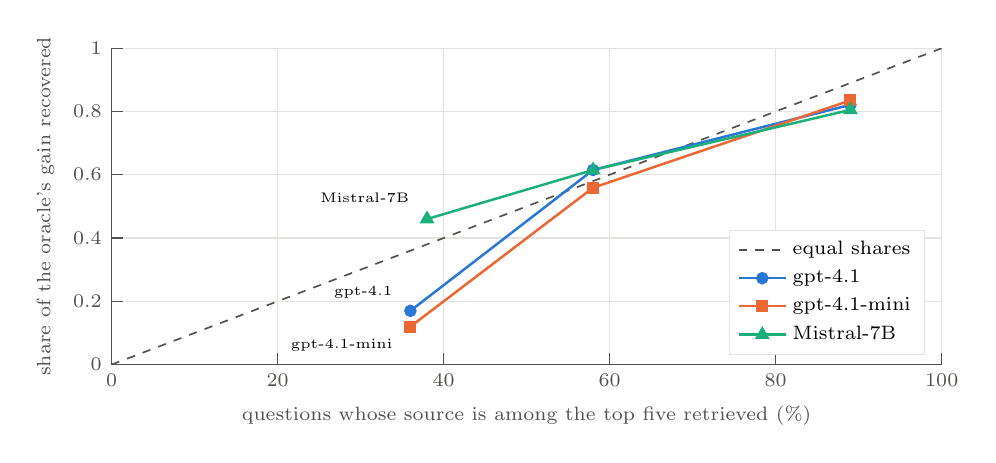
\begin{tikzpicture}
\begin{axis}[
  width=\columnwidth, height=5.6cm,
  xmin=0, xmax=100, ymin=0, ymax=1,
  xtick={0,20,40,60,80,100}, ytick={0,0.2,0.4,0.6,0.8,1},
  xticklabel style={font=\scriptsize, text=inkmuted},
  yticklabel style={font=\scriptsize, text=inkmuted, /pgf/number format/fixed, /pgf/number format/precision=1},
  xlabel={questions whose source is among the top five retrieved (\%)},
  ylabel={share of the oracle's gain recovered},
  label style={font=\scriptsize, text=inkmuted},
  axis line style={draw=inkmuted, line width=0.4pt},
  tick style={draw=inkmuted, line width=0.4pt},
  major grid style={draw=gridline, line width=0.4pt},
  ymajorgrids, xmajorgrids,
  axis x line*=bottom, axis y line*=left,
  legend style={at={(0.98,0.03)}, anchor=south east, font=\scriptsize, draw=gridline, fill=white,
                text=black, row sep=0pt},
  legend cell align=left,
  every axis plot/.append style={line width=0.9pt},
]
\addplot[color=inkmuted, dashed, line width=0.6pt] coordinates {(0,0) (100,1)};
\addlegendentry{equal shares}
\addplot[color=seriesA, mark=*, mark size=1.8pt] coordinates {(36,0.17) (58,0.615) (89,0.821)};
\addlegendentry{gpt-4.1}
\addplot[color=seriesB, mark=square*, mark size=1.7pt] coordinates {(36,0.12) (58,0.559) (89,0.835)};
\addlegendentry{gpt-4.1-mini}
\addplot[color=seriesC, mark=triangle*, mark size=2.2pt] coordinates {(38,0.46) (58,0.615) (89,0.805)};
\addlegendentry{Mistral-7B}
\node[font=\tiny, text=black, anchor=south east] at (axis cs:35,0.18) {gpt-4.1};
\node[font=\tiny, text=black, anchor=north east] at (axis cs:35,0.11) {gpt-4.1-mini};
\node[font=\tiny, text=black, anchor=south east] at (axis cs:37,0.48) {Mistral-7B};
\end{axis}
\end{tikzpicture}
\caption{The share of the oracle's gain over closed-book that plain RAG recovers, on the same questions,
against the share of questions whose source reaches the context (gpt-4.1 judge): \dq{} on an earlier,
unfrozen pool (36--38\%, indicative), on the frozen pool (58\%), and \fresh{} (89\%).}
\label{fig:recall}
\end{figure}

\subsection{RQ4: Dewey on RAGScholar's questions}
\label{sec:rq4}

\begin{table*}[t]
\caption{Dewey on \dq{} and \fresh{} (gpt-4.1 judge): mean score with 95\% interval, and paired
differences from the study's runs on the same questions. RAGScholar configuration: Mistral-7B, BM25 top
five concatenated, on the frozen pool. Source given: questions whose source abstract reached Dewey.}
\label{tab:dewey}
\centering\footnotesize
\setlength{\tabcolsep}{3pt}
\begin{tabular}{llcccccc}
\toprule
Set & Dewey & Mean & vs closed-book & vs plain RAG & vs RAGScholar & Source & Median \\
 & & & (gpt-4.1-mini) & (gpt-4.1-mini) & configuration & given & seconds \\
\midrule
\dq{} & before the content tool & \pending{} & \pending{} & \pending{} & \pending{} & -- & \pending{} \\
 & as deployed & \pending{} & \pending{} & \pending{} & \pending{} & \pending{} & \pending{} \\
 & on the frozen pool & \pending{} & \pending{} & \pending{} & \pending{} & \pending{} & \pending{} \\
\midrule
\fresh{} & before the content tool & \pending{} & \pending{} & \pending{} & \pending{} & -- & \pending{} \\
 & as deployed & \pending{} & \pending{} & \pending{} & \pending{} & \pending{} & \pending{} \\
 & on the frozen pool & \pending{} & \pending{} & \pending{} & \pending{} & \pending{} & \pending{} \\
\bottomrule
\end{tabular}
\end{table*}

\pending{Dewey results: levels, the three contrasts, the decomposition into model and agent, citations,
how often it searched and with which query, cost and latency.}

\subsection{RQ5: Questions about dblp's records}
\label{sec:rq5}

\begin{table}[t]
\caption{Seventy questions about dblp's records, scored by exact match against values computed from the
dump: correct answers per kind (of 10).}
\label{tab:structured}
\centering\scriptsize
\setlength{\tabcolsep}{2.6pt}
\begin{tabular}{lcccc}
\toprule
 & & \multicolumn{2}{c}{RAGScholar-style} & No retrieval \\
\cmidrule(lr){3-4}
Kind & Dewey & gpt-4.1-mini & Mistral-7B & gpt-4.1-mini \\
\midrule
Paper: venue and year & \pending{} & \pending{} & \pending{} & \pending{} \\
Paper: authors & \pending{} & \pending{} & \pending{} & \pending{} \\
Person: publications & \pending{} & \pending{} & \pending{} & \pending{} \\
Venue: papers in a year & \pending{} & \pending{} & \pending{} & \pending{} \\
Venue: top author & \pending{} & \pending{} & \pending{} & \pending{} \\
Two people: joint papers & \pending{} & \pending{} & \pending{} & \pending{} \\
Name: different people & \pending{} & \pending{} & \pending{} & \pending{} \\
\midrule
All (70) & \pending{} & \pending{} & \pending{} & \pending{} \\
\bottomrule
\end{tabular}
\end{table}

\pending{record-question results and the sign test against each arm}

\subsection{RQ6: Robustness to the grading and the judge}
\label{sec:rq6}

\textbf{Single-reference grading.} On the 21 \dq{} questions whose source was missed, graded against the
reference, the GPT models fall slightly below their closed-book scores (gpt-4.1-mini $-0.14$, gpt-4.1
$-0.05$; Table~\ref{tab:missed}), while Mistral-7B gains ($+0.14$). An audit of the 98 answers that lost
points on these questions (two labellers, $\kappa=0.78$) labels 75 of them a correct answer to the
question as worded, supported by an abstract of a different paper; these labels proved generous on
\fresh{}, so we rely on a controlled re-grade. All twelve answer sets on the 21 missed questions are graded
again by a multi-reference judge: the same gpt-4.1, shown the reference and the same five retrieved
abstracts for every answer, credits any answer that is correct for the question as worded, whether
supported by an abstract or by established knowledge. It must first pass three controls: the reference
scores 2 (21/21), another question's reference scores 0 (20/21), and another question's RAG answer scores
0 (21/21). The evidence is common but does not work alike for all answers: a RAG answer can be checked
against the abstracts it paraphrases, a closed-book answer only against the judge's own knowledge.

\begin{table*}[t]
\caption{The 21 \dq{} questions whose source was missed: mean score graded against the single reference,
and re-graded by the multi-reference judge (gpt-4.1), with the paired difference from the same model's
closed-book answers graded the same way (95\% interval; questions better/worse).}
\label{tab:missed}
\centering\small
\begin{tabular}{llcccc}
\toprule
Model & Condition & \multicolumn{2}{c}{Single reference} & \multicolumn{2}{c}{Multi-reference re-grade} \\
\cmidrule(lr){3-4}\cmidrule(lr){5-6}
 & & Mean & $\Delta$ & Mean & $\Delta$ \\
\midrule
gpt-4.1 & closed-book & 1.52 & & 1.81 & \\
 & RAG & 1.48 & $-$0.05 & 1.71 & $-$0.10 \ci{$-$0.33}{$+$0.14} (2/4) \\
 & permissive & 1.62 & $+$0.10 & 1.91 & $+$0.10 \ci{0.00}{$+$0.24} (2/0) \\
 & gated & 1.38 & $-$0.14 & 1.76 & $-$0.05 \ci{$-$0.29}{$+$0.14} (2/3) \\
\midrule
gpt-4.1-mini & closed-book & 1.52 & & 1.71 & \\
 & RAG & 1.38 & $-$0.14 & 1.67 & $-$0.05 \ci{$-$0.24}{$+$0.14} (2/3) \\
 & permissive & 1.38 & $-$0.14 & 1.67 & $-$0.05 \ci{$-$0.24}{$+$0.14} (2/3) \\
 & gated & 1.24 & $-$0.29 & 1.67 & $-$0.05 \ci{$-$0.29}{$+$0.14} (2/3) \\
\midrule
Mistral-7B & closed-book & 1.14 & & 1.33 & \\
 & RAG & 1.29 & $+$0.14 & 1.43 & $+$0.10 \ci{$-$0.24}{$+$0.43} (6/5) \\
 & permissive & 1.14 & 0.00 & 1.57 & $+$0.24 \ci{$-$0.05}{$+$0.52} (6/2) \\
 & gated & 1.14 & 0.00 & 1.52 & $+$0.19 \ci{$-$0.10}{$+$0.48} (5/2) \\
\bottomrule
\end{tabular}
\end{table*}

Re-grading credits closed-book answers too (gpt-4.1: $1.52\rightarrow1.81$), so the audit alone would have
overstated retrieval. Under the multi-reference grade, no condition differs detectably from closed-book on
the missed questions: every difference for the GPT models lies within $\pm0.10$ with an interval spanning
zero, and Mistral-7B's are positive ($+0.10$ to $+0.24$) with intervals that touch zero. Most of the
single-reference loss is therefore a grading artefact, although some answers still got worse (4 of 21 for
gpt-4.1's plain RAG), and 21 questions cannot rule out a modest cost.

\textbf{A second judge.} gpt-4.1 grades answers from its own model family, and LLM judges can prefer their
own generations~\cite{panickssery2024selfpref}. Qwen2.5-14B-Instruct, served on the same CPU machine,
re-grades the closed-book, plain RAG and oracle sets of all three models on \dq{}, after passing the same
controls (50/50 and 50/50). The judges agree on 359 of 438 answers (82\%; Cohen's $\kappa=0.49$,
quadratic-weighted $\kappa=0.76$~\cite{cohen1968weighted}); 70 of the 79 disagreements are between 1 and
2. Qwen is more lenient with closed-book answers and stricter with answers built on abstracts (Mistral-7B
with RAG: 1.60 and 1.32). There is no sign of self-preference in single-reference grading: the gap between
the judges is $-0.05$ for gpt-4.1's answers and $+0.02$ for gpt-4.1-mini's, but $+0.14$ for Mistral-7B's.

\begin{table}[t]
\caption{Paired differences from closed-book on \dq{} under the primary judge (gpt-4.1) and the second
judge (Qwen2.5-14B), graded against the single reference, and for the missed questions also by each
judge's multi-reference re-grade (multi-ref.). Bold: the 95\% interval excludes zero.}
\label{tab:judges}
\centering\footnotesize
\setlength{\tabcolsep}{3pt}
\begin{tabular}{llcc}
\toprule
Model & Contrast (questions) & gpt-4.1 & Qwen2.5-14B \\
\midrule
gpt-4.1 & RAG, all (50) & \textbf{$+$0.30} & $+$0.06 \\
 & RAG, source retrieved (29) & \textbf{$+$0.55} & \textbf{$+$0.31} \\
 & RAG, source missed (21) & $-$0.05 & $-$0.29 \\
 & \quad multi-ref. & $-$0.10 & $+$0.10 \\
 & Oracle (46) & \textbf{$+$0.52} & \textbf{$+$0.33} \\
\midrule
gpt-4.1-mini & RAG, all (50) & \textbf{$+$0.32} & $-$0.02 \\
 & RAG, source retrieved (29) & \textbf{$+$0.66} & \textbf{$+$0.24} \\
 & RAG, source missed (21) & $-$0.14 & \textbf{$-$0.38} \\
 & \quad multi-ref. & $-$0.05 & $-$0.14 \\
 & Oracle (46) & \textbf{$+$0.59} & \textbf{$+$0.26} \\
\midrule
Mistral-7B & RAG, all (50) & \textbf{$+$0.56} & $+$0.24 \\
 & RAG, source retrieved (29) & \textbf{$+$0.86} & \textbf{$+$0.66} \\
 & RAG, source missed (21) & $+$0.14 & $-$0.33 \\
 & \quad multi-ref. & $+$0.10 & $-$0.29 \\
 & Oracle (46) & \textbf{$+$0.96} & \textbf{$+$0.74} \\
\midrule
Dewey & \pending{as deployed, vs closed-book} & \pending{} & \pending{} \\
 & \pending{vs RAGScholar configuration} & \pending{} & \pending{} \\
\bottomrule
\end{tabular}
\end{table}

Table~\ref{tab:judges} separates what holds from what does not. Under both judges, the oracle and RAG with
the source retrieved improve significantly on closed-book for every model. On the missed questions,
graded against the single reference, Qwen penalises answers built on the wrong papers more heavily ($-0.29$
to $-0.38$, significant for gpt-4.1-mini), which cancels the net gain of plain RAG for the GPT models
($+0.06$ and $-0.02$). Qwen also passes the multi-reference re-grade's three controls (21/21 each) and,
crediting any correct answer, finds no detectable difference from closed-book for any model: $+0.10$ for
gpt-4.1, $-0.14$ for gpt-4.1-mini and $-0.29$ for Mistral-7B, all with intervals spanning zero. The one
significant harm disappears, but the judges still differ: their estimates for gpt-4.1's answers lie on
opposite sides of zero ($-0.10$ and $+0.10$), Mistral-7B's estimate under Qwen barely moves (2 answers
better, 8 worse), and the levels differ (Mistral-7B's RAG answers: 1.43 and 0.91). What retrieving the
wrong papers appears to cost depends on the grading protocol and on the judge. The controls also guarded
the protocol: placing the answer after the abstracts, which runs five times faster on a local judge, made
gpt-4.1 score two of 21 mismatched references above zero (19/21), so both judges use the original order.

%% ===================================================================================================
\section{Discussion}

\textbf{What \dq{} measures.} With current models, \dq{} measures three things: whether the source
abstract is retrieved; how much the model knows about the field, which on a set where 58\% of questions
are general knowledge is a great deal; and how the grader treats correct answers that are not the
reference answer. Generation from the right abstract is near the ceiling under the primary judge on both
sets, and we find no sign that the models' knowledge comes from memory of the papers, although 20
identifiable \dq{} questions cannot rule out a modest effect.

\textbf{Dewey against RAGScholar.} \pending{what is better and why: on its own task (model, retrieval,
agent), on records (scope), attribution (citations, lookups shown), reproducibility; what is not.}

\textbf{Recommendations for scholarly RAG benchmarks.} Report closed-book and oracle conditions next to
retrieval, so that prior knowledge and the generation ceiling are visible. Evaluate retrieval in an open
world, by the rate at which the source reaches the context. Grade against multiple references, or with a
judge that may credit other correct answers under controls, and report results under at least two judges
from different families. Prefer questions that identify their paper: on \dq{} itself, plain RAG adds 0.50
to 0.90 points on identifiable questions but only 0.14 to 0.28 on general ones (Table~\ref{tab:audit}).
And ask questions about records too: a bibliography is queried for more than paper content.

\textbf{Limitations.} Fifty questions give wide intervals, and subgroup analyses wider still. The original
models were sampled once per question at temperature~0.7, and quantised. Every content grade comes from an
LLM judge; controls, inter-labeller agreement, the multi-reference re-grade and the second judge bound but
do not remove that dependence, the two judges differ in level, and no human ratings were collected.
\fresh{}'s questions and references were written by gpt-4.1, which also grades them and answers some of
them, and a 2025 paper may have had an earlier preprint. The memory comparison rests on 20 identifiable
\dq{} questions against 84 \fresh{} ones built differently. Our open-world pools depend on public services,
one of which refused most searches, and BM25 uses pool-level statistics. Dewey's content tool and prompt
were designed on the same questions it is evaluated on; the record questions and their scoring were fixed
before any system answered them. Dewey's gold set and scenarios were written by its developer.

\textbf{Future work.} Human ratings of a sample of the answers on which the judges disagree; multiple
reference answers per \dq{} question; questions that describe papers in other words, on which the ranker
should be compared again; and real users' questions.

%% ===================================================================================================
\section{Conclusion}

\pending{rewrite once the Dewey results are in}

\section*{Acknowledgment}

The author thanks the creators of RAGScholar and DBLP-QA for releasing their dataset, and the dblp,
OpenAlex and Semantic Scholar teams for their open data and services. Language models are the object of
this study and part of Dewey: they answer the questions, write the \fresh{} questions, grade the answers,
label the questions and gate the retrieved abstracts, as described above. In addition, an AI assistant
(Claude, Anthropic) was used to implement Dewey and the evaluation harness and to draft the text; the
author reviewed and edited the content and takes full responsibility for it.

\bibliographystyle{IEEEtran}
\bibliography{references}

\appendix[Prompts]
\label{app:prompts}

\textbf{Closed-book.} \emph{System:} ``You answer questions about computer-science research. Answer in
one to three sentences.'' \emph{User:} the question.

\textbf{Oracle and single abstracts (A1--A5).} \emph{System:} ``You answer questions about computer-science
research using the [paper] abstract you are given. Answer in one to three sentences.'' \emph{User:}
``Abstract: \ldots{} Question: \ldots''

\textbf{RAG (Top-$k$-CD) and gated.} As the oracle, with ``the paper abstracts you are given'' and the
numbered, titled abstracts.

\textbf{Concatenated answers (Top-$k$-CA).} ``You answer questions about computer-science research. You
are given answers to the question, each written from the abstract of one paper a search returned. Combine
them into one answer, in one to three sentences.'' The answers are the same model's A1--A$k$ answers.

\textbf{RAG permissive.} ``You answer questions about computer-science research. You are given
abstracts of papers a search returned for the question; they may or may not be relevant. Use them where
they address the question; if none does, ignore them and answer from your own knowledge. Answer in one
to three sentences.''

\textbf{Gate.} ``You check search results for a question about computer-science research. You are given
the question and numbered paper abstracts. Say which abstracts contain information that answers the
question; an abstract on the same broad topic that does not address what is asked does not count.''

\textbf{Answer-bearing check.} ``You check whether one paper abstract answers a question about
computer-science research. You are given the question, its ground-truth answer, and the abstract. Say true
if the abstract itself states what the ground-truth answer says, in any wording, so that someone who read
only this abstract could answer the question correctly.''

\textbf{RAGScholar-style pipeline on records.} ``You answer questions about computer-science papers using
the search results you are given: each has its dblp key, DOI, title, authors, year and abstract. Answer in
one to three sentences.''

\textbf{Dewey's content rule.} ``Questions about what papers say [\ldots] are answered with
search\_abstracts. Pass the question as the user asked it, made self-contained [\ldots]. Answer from the
returned abstracts, and end every sentence that uses one with its number in brackets [\ldots]. If none of
them addresses the question, say so in one clause; you may then add one or two sentences of general
background, saying that it is general background, with no numbers and no citations.''

\textbf{Question writer (\fresh{}).} ``You write questions for a benchmark about computer-science
research, the way its authors did. You are given one paper's abstract. Write one question that the
abstract answers, about the paper's main idea, method, finding or motivation, and its answer: one to
three sentences taken from the abstract. The question must make sense on its own.''

\textbf{Judge.} The benchmark's 0--2 scale with the original paper's worked example (its Table~2); it
grades only against the reference, does not penalise extra correct detail, and does not reward fluency.

\textbf{Multi-reference judge.} A 0--2 scale without the worked example, with the reference and the five
retrieved abstracts (the answer to grade precedes the abstracts): 2 if the answer matches the reference
\emph{or} is an equally valid answer to the question as worded, supported by one of the abstracts or by
established knowledge.

\end{document}
